\documentclass[MASTER.tex]{subfiles} 
\begin{document} 
%============================================================ %

\begin{frame}[fragile]
	\Large
	Some of these packages also have functions to explore patterns of missingness % (e.g., missing.pattern.plot() in the mi package).

	\begin{itemize}	
	\item \textbf{Amelia II:} A Program for Missing Data
	\item \textbf{Hmisc:} Harrell Miscellaneous
	\item \textbf{mi:} Missing Data Imputation and Model Checking
	\item \textbf{mitools:} Tools for multiple imputation of missing data
	\end{itemize}
\end{frame}	
\begin{frame}
	\begin{figure}
\centering
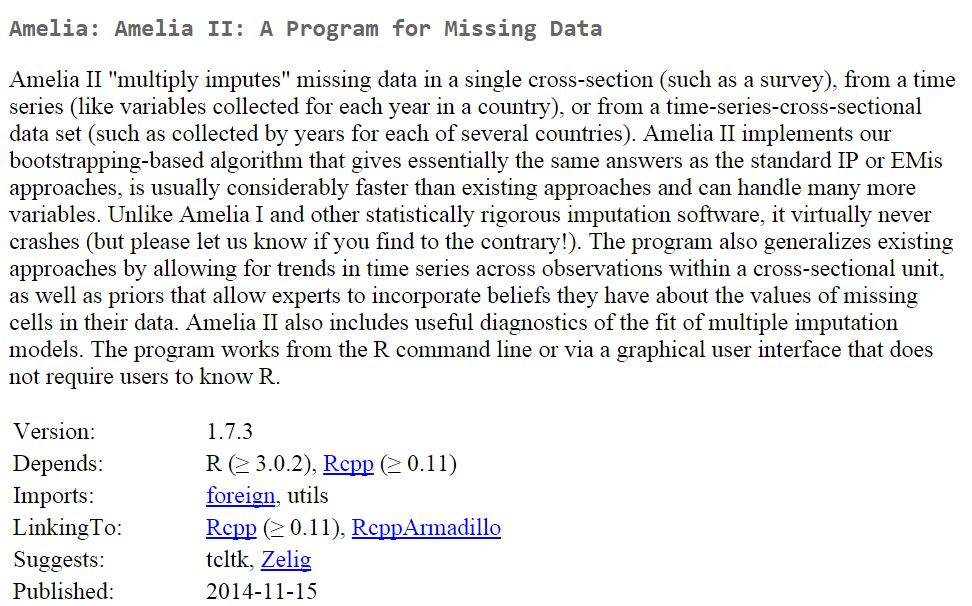
\includegraphics[width=1.1\linewidth]{C:/Users/Kevin/Documents/GitHub/TidyRMissingData/CRAN-Amelia}
\end{figure}
\end{frame}
%============================================================ %
\begin{frame}
	\begin{figure}
\centering
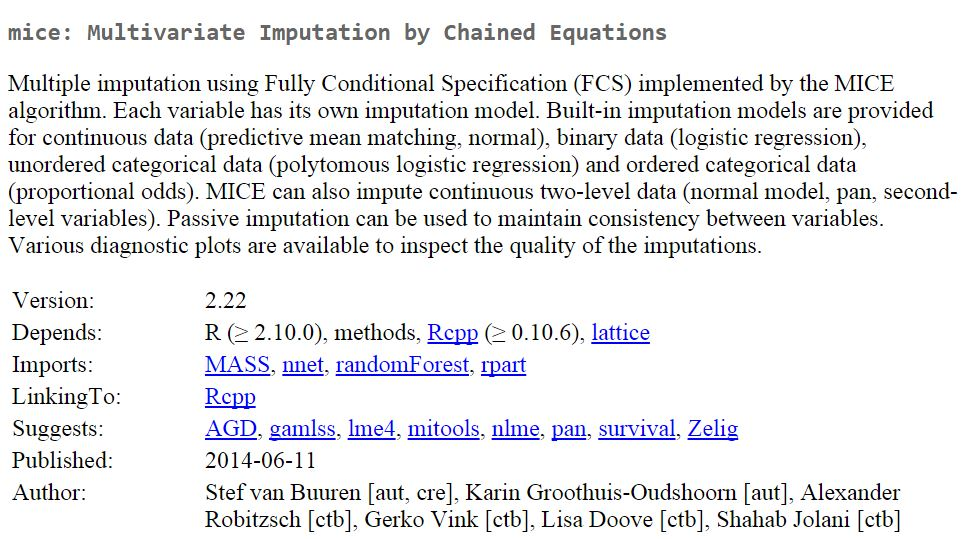
\includegraphics[width=1.1\linewidth]{C:/Users/Kevin/Documents/GitHub/TidyRMissingData/CRAN-MICE}
\end{figure}
\end{frame}
%============================================================ %
\begin{frame}
	\begin{figure}
\centering
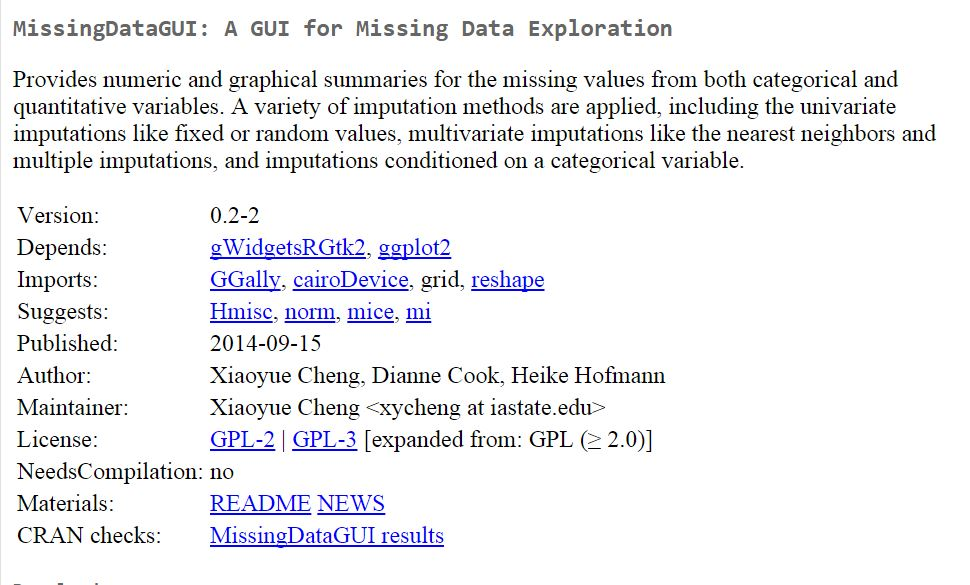
\includegraphics[width=1.1\linewidth]{C:/Users/Kevin/Documents/GitHub/TidyRMissingData/CRAN-MissingDataGUI}
\end{figure}
\end{frame}
%============================================================ %
\begin{frame}
\begin{figure}
\centering
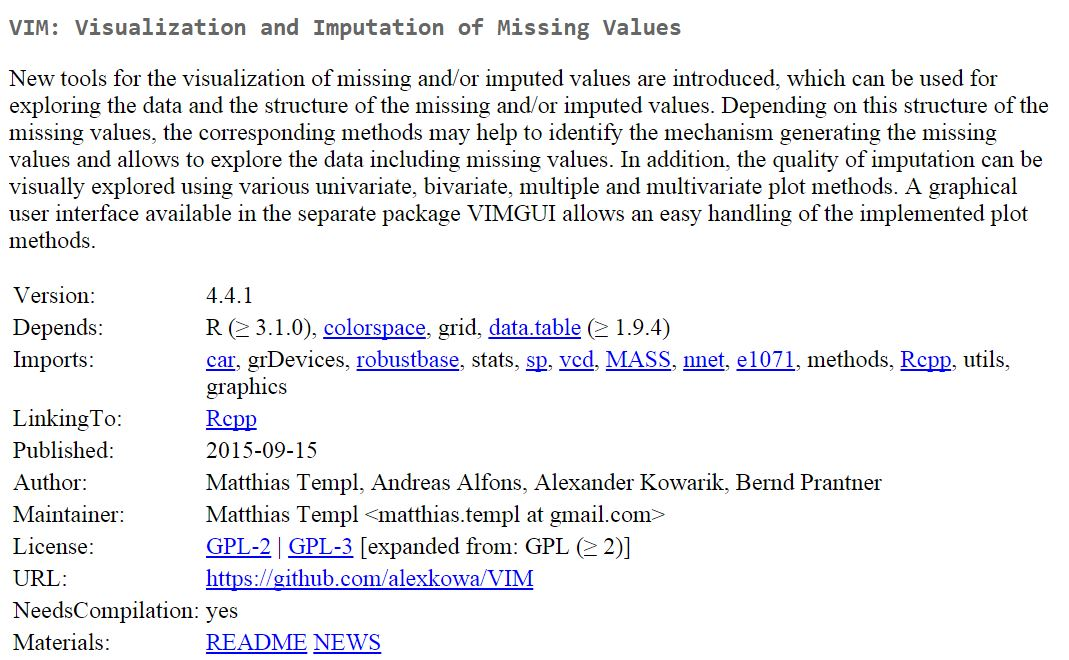
\includegraphics[width=1.1\linewidth]{CRAN-vim}
\end{figure}
\end{frame}
%============================================================ %

\end{document}